\newcommand{\CLASSINPUToutersidemargin}{1.5in}
\documentclass[10pt,final,journal]{IEEEtran}
\usepackage{graphicx}

\begin{document}
\title{Troups: Scalable Group Transactions for BigTable datastores}
\author{Benjamin Busjaeger, Jonathan Chu, Daniel Ormond \\
\{busjaeg2, jmchu2, ormond1\}@illinois.edu}
\date{Feb 2012}
\maketitle

\begin{abstract}
Troups is a novel transaction manager for cloud datastores of the BigTable family that provides full ACID transactions for groups of co-located data items.

This allows us to improve the consistency guarantees without significantly impacting the high scalability or availability of these systems. We have also implemented a learning algorithm that derives groupings of entities from transaction logs to optimize data co-location for transaction processing.
\end{abstract}

\begin{IEEEkeywords}
cloud, data storage, BigTable, transaction processing, partitioning
\end{IEEEkeywords}

\section{Introduction}
Cloud platforms like Google and Amazon store vast amounts of data. This is in part because they pool resources to efficiently serve multiple tenants and in part because the volume of data produced by applications and users has significantly increased in recent years. At the same time users expect their data to always be quickly accessible anywhere and they have little tolerance for data loss or inconsistencies. Studies like ~\cite{Ramsay:1998} have shown that users quickly become  irritated by long response times and take their business elsewhere. Unfortunately, per Brewer's conjecture ~\cite{gilbert2002brewer}, it is not possible to maximize all of these goals simultaneously. The challenges have forced a change in the way data is stored and processed in the cloud.

Traditional relational database management systems (RDBMSs) are designed to provide high consistency by giving users the impression of a single system image. The conventional approach to improving availability and performance of these systems has been to buy more powerful and resilient hardware. This has obvious scalability limitations and is often not cost effective. The alternative of clustering traditional RDBMSs across less expensive hardware has its own set of challenges, since the single system objective implies high overhead from frequent distributed transactions and limited partition tolerance. Popular open source databases like MySQL have been shown to only scale to a small number of nodes ~\cite{Malkowski:2010:EAD:1774088.1774449} and commercial RDBMSs have similar limitations ~\cite{Campbell:2010:ESF:1807167.1807280}.

In response to the lack of scalability and high operational cost of traditional RDBMSs, large Internet companies have recently developed their own data storage solutions. Some notable examples of these so called NoSQL datastores are Google's BigTable ~\cite{Chang:2006:BDS:1267308.1267323}, Yahoo's PNUTS ~\cite{Cooper:2008:PYH:1454159.1454167}, and Amazon's Dynamo ~\cite{DeCandia:2007:DAH:1323293.1294281}. These architectures are radical departures from traditional RDBMSs in that they do not expose complex query operations and provide only limited consistency guarantees. This allows them to more efficiently partition data across dynamically scalable clusters and to isolate faults to subsets of the system.

Many cloud applications, like search index construction, can easily tolerate relaxed consistency guarantees. However, other applications, like emerging OLTP multi-tenant platforms, have strong isolation and atomicity requirements. Without sufficient transaction support built into the infrastructure, the burden of ensuring data integrity is ultimately placed on application developers.

Troups aims to improve the transactional capabilities of NoSQL datastores in the BigTable family without significantly impacting their high availability and scalability. Concretely, it adds lock-free ACID transactions across co-located data items. It also includes fault-tolerant distributed transactions, but tries to minimize their use through optimized data placement. The idea as such is not new, but the way in which Troups realizes it is. In summary, our main contributions to the research field are:

\begin{enumerate}
\item A novel transaction manager for BigTable-like datastores. This transaction manager is only loosely coupled with BigTable, so it is likely applicable to other datastores.
\item A mechanism to group related rows along with an algorithm to automatically detect row groups from transaction logs.
\item A timestamp service and protocol useful for implementing multiversion or timestamp-based concurrency control protocols in distributed systems.
\item An extensible and open implementation of these components on top of HBase \footnote{http://hbase.apache.org/}.
\end{enumerate}

\section{Related Work}
		
\subsection{OLTP Cloud Datastores}
\emph{Cloud SQL Server} ~\cite{Campbell:2010:ESF:1807167.1807280, Bernstein:2011:AMS:2004686.2005651}, \emph{ElasTraS} ~\cite{Das:2009:EET:1855533.1855540, Das:2010:EAE}, and \emph{Relational Cloud} ~\cite{Curino:2011:JPMWMBZ11} describe approaches for horizontally scaling out different relational DBMSs. Cloud SQL Server augments Microsoft SQL Server with partitioning and primary-copy replication. Serializable ACID transactions are supported, but limited to a single partition. A partition can be a whole logical database, referred to as a table group, if it is sufficiently small, or a set of rows from a table group that have been assigned a common partitioning key by the user in the database schema. ElasTraS uses hierarchical schema-level partitioning and also restricts transactions to one partition. It differs from Cloud SQL Server in that it decouples storage from metadata management through the use of a distributed file system. This allows for a dynamic mapping between partitions and nodes. Relational Cloud combines a workload-aware approach for efficient data placement with a graph-based partitioning algorithm for data co-location discussed in the next section. ACID transactions are supported within and across partitions. Although our approach is not targeted at RDBMSs, it uses similar partitioning techniques.

\emph{Percolator} ~\cite{Peng:2010:LIP:1924943.1924961}, \emph{HBaseSI} ~\cite{Zhang:2010:5697970} and \emph{ReTSO} ~\cite{Junqueira:2011:LTS:2056318.2057148} are different approaches for adding global transactions with snapshot isolation \footnote{See Background section for details on snapshot isolation} semantics to BigTable-like datastores. Percolator is specifically designed to allow incremental search index construction, so it is optimized for throughput and not suitable for latency-sensitive applications. HBaseSI is a pure client API that uses a set of custom tables and atomic test-and-set operations to manage transactions without central coordination. ReTSO implements a lock-free commit algorithm using a centralized Transaction Status Oracle. The benefit of these approaches is that they do not rely on data co-location to support one-phase commit transactions. The downside is weaker isolation. Troups's transaction manager supports serializable and snapshot isolation, although only the former is currently implemented, and it is neither fully decentralized nor centralized. It builds on some of the ideas presented in ReTSO to implement non-invasive and efficient multiversion concurrency control.

\emph{G-Store} ~\cite{Das:2010:GSD:1807128.1807157} and \emph{CloudTPS} ~\cite{Wei:2011:5740834} build transaction capabilities targeted at specific use cases on top of BigTable-like datastores. G-Store introduces a key group protocol to provide ACID transactions over a dynamically selected set of keys. It is intended for applications which need to execute transaction across frequently changing groups of entities, that are non-overlapping, so it has limited applicability. CloudTPS is designed for web application workloads and assumes short-lived transactions that access small data sets known prior to starting the transaction. It interposes a group of Local Transaction Managers (LTMs) between clients and datastores which load data items and transaction state into memory for efficient processing. This implies the need for a separate server cluster with its own fail-over and recovery mechanisms.

\emph{MegaStore} ~\cite{Furman:2008:8530095, Baker:2011:8530095} also tries to bridge the gap between RDBMSs and NoSQL datastores by providing strong consistency guarantees within fine-grained partitions. It also builds on BigTable and its transaction manager employs multiversion concurrency control and supports distributed transactions. As such, it is most closely related to our work. Nevertheless, there are several differences that distinguish the systems. First, the design center of Megastore is on high availability through synchronous cross-data center replication. Troups targets low-latency intra-data center transaction processing and relies on BigTable's default replication strategy. Furthermore, Megastore provides a declarative schema language with support for secondary indices, whereas Troups uses the BigTable data model. Data groups in Megastore are statically declared in the schema at design-time, whereas in Troupss they are dynamically computed based on a user-defined grouping function. The transaction managers in the two systems also differ in several aspects. In Megastore the group is the unit of concurrency control and logging to enable wide-area network replication. Mutations are first appended to the replicated log and then applied to the datastore after the commit. Reads within groups block until changes are applied, whereas reads across groups may not see the latest committed data. In Troups the unit of concurrency control is an individual cell and the log is tablet-scoped. This enables a high degree of concurrency and batch commit optimizations across groups. Mutations are directly written into the datastore and filtered for read operations. Therefore, readers can see the last written mutation, even if it has not been committed yet.

\emph{Deuteronomy} ~\cite{Levandoski:2011:8530161} is noteworthy, because it aims to decouple transaction management from the underlying datastore, a goal shared by our work. To this end, it defines a transaction component (TC) capable of providing full ACID transactions for any datastore that implements a well-defined data component (DC) interface. The TC applies concurrency control and undo/redo logging at the logical record level as opposed to at the physical page level. Our transaction manager also operates against an abstract datastore contract. Our approach differs from Deuteronomy in that it uses different concurrency control and recovery algorithms and does not rely on a centralized transaction manager.

Table ~\ref{classification} summarizes the classification discussed above.

\begin{table}[!t]
\renewcommand{\arraystretch}{1.3}
\caption{OLTP Cloud Data Store Classification}
\label{classification}
\centering
\begin{tabular}{|c|c|c|c|}
\hline
\bfseries Data Store  & \bfseries Data Model & \bfseries  Part. & \bfseries Isolation \\
\hline
\hline
Cloud SQL & relational & yes & serializable \\
ElasTraS & relational & yes & serializable \\
Rel. Cloud & relational & yes & serializable \\
Percolator & BigTable & no & snapshot \\
HBaseSI & BigTable & no & snapshot \\
ReTSO & BigTable & no & snapshot \\
G-Store & BigTable & yes & serializable \\
CloudTPS & BigTable & no & serializable \\
Megastore & BigTable & yes & serializable \\
Deuteronomy & agnostic & no &serializable \\

\hline
\end{tabular}
\end{table}

\subsection{Paritioning Algorithms}
There are multiple partitioning algorithms in use and in study currently.  Not all of the algorithms have the same goal.  Hash-based algorithms help scale the database by evenly distributing the data on different nodes while other algorithms have a more specific goal to reduce transaction overhead.

Schism ~\cite{Curino:2010:SWA:1920841.1920853} is a static partitioning algorithm to reduce distributed transactions for SQL datastores. It uses transaction logs to determine how to partition data. The transaction anaylsis is similar to the work done by Chun-Hung et al.~\cite{chun:2002} It significantly improves performance compared to hash-based and even manual partitioning techniques. These static algorithms are a good starting point for our work and would likely yield better results for key/value stores given their simplified data access model. Also, an incremental version of these algorithms may scale better than the static equivalent, since it may be able to consider only new transaction log entries in each iteration. Another option would be to use a probabilistic algorithm.

Hehme and Bruno ~\cite{Nehme:2011:APD:1989323.1989444} present and algorithm that deeply integrates directly with the parallel query optimizer in Microsoft SQL Server.  Their algorithm provides a static data partitioning recommendation.  Their goals was to provide a data partition strategy in less time than other less deeply integrated solutions.


\section{Background}

\subsection{BigTable}
BigTable ~\cite{Chang:2006:BDS:1267308.1267323} is a distributed storage system developed by Google to efficiently store large amounts of data (petabytes) across many machines (1000s). Data is stored in tables, which are multidimensional maps that index values by a triple consisting of row key, column key, and timestamp. Tables are sparse, meaning only cells that contain data are persisted, and they are sorted in lexicographical order by row key. Each table is dynamically partitioned into ranges of rows, called \emph{tablets}, which are assigned to \emph{tablet servers} by a dedicated \emph{master}. Tablets are reassigned in case of server failure or overload and they are automatically split or merged with other tablets if their size exceeds or falls below certain thresholds. \emph{Clients } access data by first looking up the locations of tablet servers that currently serve the tablets containing relevant rows and then issuing operations against these tablet servers. If the row locations change in between these two steps, the client retries.

Supported operations include read, write, and delete for single rows, batch operations across rows, and scanners with filters to iterate over a subset of rows. The server-side scripting language Sawzall ~\cite{Pike:2005} can be used for more complex read-only queries. Single-row operations are atomic and transactions across multiple single-row operations are also supported. Note that this can be supported efficiently in this model, since data in a single row is always stored on the same tablet server. Transactions for operations that span multiple rows are not supported.

Tablets are physically stored in the Google File System (GFS) ~\cite{Ghemawat:2003:GFS:1165389.945450} as large immutable SSTable files. To make small mutations efficient, BigTable first writes them into a redo log and then stores them in an in-memory data structure called \emph{memtable}. The memtable is periodically written to new SSTables and SSTables are iteratively merged through a \emph{compaction} process. The redo log is scoped to tablet servers to reduce disk seeks, so if a tablet server crashes, the log has to be split across tablet servers that are assigned to recover the tablets. Recovery consists of replaying any mutations that have not be stored in SSTables into the new memstore. To avoid this overhead when moving tablets between servers, the source server compacts the tablet once before and once after closing.

BigTable was recently enhanced with Coprocessors which allow executing code directly on tablet servers similar to stored procedures in traditional database systems ~\cite{Dean:2009}. Coprocessors are attached to tablets and share their lifecycle. Clients can invoke coprocessors through a high-level call interface that resolves the location of Coprocessors based on rows. HBase, the main open source implementation of BigTable, also offers Coprocessor \emph{Observers}, which are not invoked by clients, but registered to receive various notifications for tablet operations. They are similar to triggers in traditional database systems.

\subsection{Multiversion Concurrency Control}
Multiversion concurrency control (MVCC) ~\cite{Bernstein:1983:MCC:319996.319998} synchronizes concurrent access to data items by having each write operation produce a new version of the data and by mapping each read operation to one of these versions. MVCC allows for a higher degree of concurrency than monoversion protocols, because reads can be served from older versions while newer ones are being created. It also facilitates recovery, since undoing a write means to simply delete the created version. These benefits come at the cost of additional storage needed to keep multiple versions around. Various MVCC protocols exist with varying degrees of isolation and different conflict resolution behavior. We will briefly discuss two relevant optimistic (non-locking) protocols.

\subsubsection{Snapshot Isolation}
In the snapshot isolation protocol ~\cite{Berenson:1995:CAS:568271.223785} each transaction is assigned a unique start timestamp that is larger than any previously assigned timestamp. Each read operation is mapped to the latest version of the data item committed before the transaction started. When a transaction commits, it receives a commit timestamp and writes a new version for each updated data item carrying this timestamps, unless a write conflict is detected, in which case it is aborted. A transaction $t_i$ is in conflict with another transaction $t_j$, if $t_j$ wrote a data item that $t_i$ also wrote and $t_j$'s commit timestamp is in the interval of $t_i$'s start and commit timestamp. This protocol allows for efficient implementation and prevents lost updates, but it does not produce serializable schedules. In particular, it does not prevent the write-skew anomaly depicted in Figure ~\ref{si} in which two transactions $t_1$ and $t_2$ first read data items $x$ and $y$ respectively and then both update the other data item.

\begin{figure}[!t]
\centering
\hspace*{-.2in}
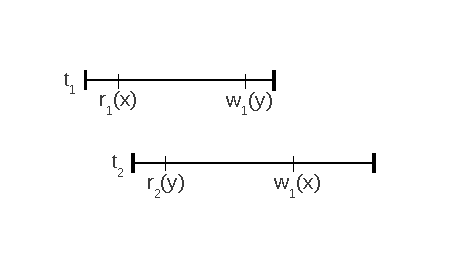
\includegraphics{images/si.pdf}
\caption{Write skew anomaly}
\label{si}
\end{figure}

\subsubsection{Multiversion Timestamp Ordering}
Multiversion timestamp ordering (MVTO) is another optimistic MVCC protocol. It assigns each transaction a unique timestamp that is larger than that of any transaction started before it. It then maps read and write operations onto versions such that the result is equivalent to that of a serial monoversion schedule in which transactions are executed in the order of their timestamps. Operations are scheduled optimistically, so if an ordering conflict occurs that cannot be resolved, one of the transactions is forced to abort and restart.

The concrete protocol consists of the following three rules ~\cite{Weikum:2001:TIS}:
\begin{enumerate}
\item A read operation of some object $x$ by transaction $t_i$ is mapped to the latest version of $x$ written by a transaction that started before $t_i$.
\item A write operation of some object $x$ is rejected and $t_i$ aborted if a transaction that started after $t_i$ has already read a version of $x$ written by a transaction that started before $t_i$. Otherwise, it is transformed into a write operation of version $i$ on object $x$.
\item A commit operation by transaction \emph{i} is delayed until all transactions that have written versions of objects read by \emph{i} have been committed.
\end{enumerate}

MVTO prevents the write-skew anomaly through the second rule: $t_1$ is forced to abort when it attempts to write a new version of $y$, since $t_2$, which started after $t_1$ has alread read the previous version. MVTO is well suited if there is little write contention and has the nice property of being deadlock free, since no locks are used and transactions only ever wait on transactions started before them to commit.

\section{Programming Model}

\subsection{Row Groups}
To enable local transactions that span multiple rows, it is necessary to co-locate them in the same tablet. Since BigTable sorts tables by row key, using a common row key prefix results in rows being placed next to each other. Such a row key prefix could be a synthetic partitioning key as used in Cloud SQL Server ~\cite{Bernstein:2011:AMS:2004686.2005651} or the key of one of the rows in the group as described in Megastore ~\cite{Baker:2011:8530095}. The latter is an obvious choice if the entities stored in the rows have an inherently hierarchical relationship. We refer to this prefix as the \emph{group key}.

We do not impose restrictions on how group keys are chosen or how they are prepended as long as the resulting key complies with the BigTable programming model. Instead, we allow users to define the mapping between row and group keys by implementing a custom table-scoped function. We call this function the  \emph{row group policy}. It is the means of declaring to the system which rows belong to the same row group. In particular, it allows the system to prevent that rows in the same grow group are separated as tablets are split. Note that this scheme preserves query granularity, since it allows for partial key scans as described in ~\cite{George:2011}.

Baker et al ~\cite{Baker:2011:8530095} also describe a pattern for merging multiple tables into a single table by prefixing column keys with table names. Combined with row grouping, this pattern makes it possible to co-locate rows from different tables. Note that such sparse tables are feasible in BigTable, since only cells that contain values are persisted.

\subsection{Group Transactions}
The client API includes methods to demarcate transaction boundaries using the familiar begin-commit-rollback idiom. When starting a new transaction, the client can either create a group or a cross group transaction. In the former case, the transaction will abort and rollback if an operation tries to access rows outside of the group accessed by previous operations within the same transaction. In the latter case, two-phase commit is used to coordinate commits across all accessed groups, which implies additional overhead, so clients should use this API sparingly.

Since Troups uses optimistic concurrency control, transactions may be aborted upon commit or even earlier if conflicts are detected that cannot be resolved. In this case, the system rolls back any changes applied by the transaction, so the client can simply retry the transaction.

Each operation must be enlisted with the transaction before it is executed. Since Troups uses the timestamp dimension to store versions created by different transactions, timestamps are not available in the client API. Note that is merely the result of an implementation choice; the system could store multiple versions under a single timestamp as described in ~\cite{Peng:2010:LIP:1924943.1924961} to preserve the timestamp dimension.

\subsection{Group Detection}


\section{Implementation}

\subsection{Timestamp Service}
The MVCC protocols used by our transaction manager require globally unique timestamps to produce serializable schedules across distributed nodes. Since storage capacity is not unlimited in practice, it also needs to know when timestamps are no longer used so that it can free up resources and clean up old versions. We encapsulate this functionality in a \emph{timestamp service (TSS)}. The basic basic function is illustrated in figure ~\ref{ts}.

\begin{figure}[!t]
\centering
\hspace*{-.2in}
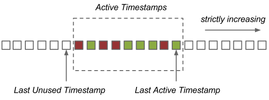
\includegraphics{images/ts-resized.png}
\caption{Timestamp service - green: active timestamps, red: released timestamps}
\label{ts}
\end{figure}

\subsubsection{Protocol}
Clients can \emph{acquire} a timestamp, which is guaranteed to be strictly greater than any currently active timestamp, but not necessarily in sequence. A client that acquires a timestamp becomes its \emph{owner}. An owner can \emph{release} a timestamp explicitly by calling the timestamp service or implicitly by failing, in which case the timestamp service eventually times out the timestamp. Clients can also query if a particluar timestamp has been released and if they are the owner of a particluar timestamp. Alternatively, clients can register to be notified when a particular timestamp has been released as a \emph{timestamp listener}. Timestamps between the last unused and first held timestamp are subject to \emph{reclamation}. In the example shown in figure ~\ref{ts} only the leftmost red timestamp is subject to reclamation. Clients can query the value of the currently last reclaimed timestamp or they can register to be notified whenever this value changes as \emph{reclamation listeners}.

While this basic protocol is sufficient if each timestamp has a single owner, it does not address the need for shared ownership, which arises when multiple clients need to hold a timestamp. To support this case, we extended the basic protocol with a \emph{participant} role. After an owner has acquired a timestamp, participants can acquire \emph{references} to it, which are uniquely identified for a particular timestamp. If the owner explicitly or implicitly releases the timestamp at this point, it is marked as released, so the semantics are the same as in the basic protocol. However, the owner can decide to \emph{persist} a set of references. After such a call, the timestamp can only be reclaimed once all participants have explicitly released their references, even if the owner releases the timestamp. In the shared protocol clients can query if a reference is held (by them) and if it is persisted. Clients can also register to be notified when a reference is released as a \emph{participant listener}.

\subsubsection{Implementation}
The timestamp service is implemented on top of Zookeeper ~\cite{Hunt:2010:ZWC:1855840.1855851}. Zookeeper is highly available and provides primitives that map directly to the timestamp protocol requirements. Basic timestamps are represented as sequential ephemeral nodes. Shared timestamps are represented as sequential persistent nodes with a special ephemeral child node to represent the owner role. References are mapped to sequential ephemeral child nodes under the timestamp. To persist a set of references, their identifiers are written into the timestamp node. When a reference is explicitly released, it's ID is removed from the timestamp node. Once all IDs have been removed, the timestamp is considered released. Watches are used to implement the various notification types.

Timestamp reclamation is performed asynchronously by a dedicated process running on one of the tablet servers. This process periodically scans timestamps until it finds an active one in an attempt to move up the last unused timestamp pointer. In the process it also deletes any shared nodes that have been released, but not properly removed. We use leader election implemented using Zookeeper to decide which tablet server should run the timestamp reclamation process at any given time.

\subsection{Transaction Manager}
Transactions are implemented by two components: a \emph{transaction client (TC)} which augments the BigTable client and a \emph{transaction manager (TM)} which augments BigTable's tablet servers. The transaction manager is a special Coprocessor that exposes transaction lifecycle operations through a Coprocessor Endpoint interface and intercepts data access operations through the Coprocessor Observer interface. As such, one instance of the transaction manager is associated with each tablet in the system and its lifecycle is tied to the tablet lifecycle.


Figure TODO illustrates how group transactions are processed. Once the first operation is enlisted with the transaction, the TC computes the group key using the row group policy specified for the table. If no row group policy is specified, each row is treated as a separate group. It then asks the TM for the row through the Coprocessor Endpoint interface to start a new transaction for the group. The TM acquires a new timestamp as the transaction identifier (TID) from the TSS, establishes the transaction state, and returns the TID to the TC. The TC annotates the operation with the returned TID before returning. On subsequent enlist calls, the TC merely checks that the row accessed by the operation is in the same row group as the row of the initial operation.

When the data access operations are submitted to the tablet server, the TM intercepts them before and after they are executed. It extracts the annotated TID to lookup the transaction state, logs the operations to enable recovery, and enforces the concurrency control protocol. This may include aborting transactions in case irresolvable conflicts are detected. When the TC receives a commit or abort, it forwards it to the TM to complete the transaction.


Cross group transactions are handled slightly differently as shown in figure TODO. The TC first acquires a shared timestamp from the TSS to use as the global TID. Whenever it receives a request to enlist a new operation, it computes the row group for it and if it has not seen it, asks the corresponding TM to join the transaction for the given group. When the TM receives a join request, it acquires a reference to the timestamp, sets a listener on the timestamp, and returns its participant ID. The TC then registers as a participant listener on the ID and returns the annotated operation. The listeners allow both the TC and TM to quickly abort the transaction in case one of them fails. Note that it is possible that the same TM is asked to join the same transaction multiple times for different groups.

When the TC receives a commit request, it initiates the two-phase commit protocol, by asking asking the TM for each row group to prepare. If only one row group was used in the transaction, the TC skips the prepare phase. If all TMs have successfully prepared, the TC persists the timestamp. At this point, a client failure will no longer result in a transaction rollback and the prepared TMs have to ensure to eventually complete the commit. The client then asks the TMs to commit their transaction branches, which result in them releasing their timestamp references. Once all TMs have completed, the TC releases the timestamp.

\subsubsection{Isolation}
At the core of the RTM is a recoverable implementation of the MVTO concurrency control protocol. The properties of MVTO make it particularly well suited for implementing transactions on top of BigTable datastores. Timestamps are already built into the data model, so they can be used to store transaction timestamps. The immutable nature of MVTO is in line with one of the core design principles underlying BigTable, namely exploiting immutability to avoid synchronization and to leverage garbage collection. Finally, BigTable is designed to dynamically scale as data grows, so it can more easily cope with the additional storage overhead for temporary versions than centralized database systems. Although our MVTO implementation is applied to HBase regions, it is designed to be datastore agnostic, so any datastore that satisfies the constraint model can be used with it.

\subsubsection{Writes}
The RTM is notified by the region whenever a row is about to be written and immediately after it was written. It processes the before-write notification by applying the second rule of the MVTO protocol for each column in the row touched by the write: If an older version of any column in the row has already been read by a younger transaction, then the current transaction is aborted. The RTM also remembers each cell written by the transaction so that it can remove them in case the transaction is aborted. Although the write itself is executed as an atomic unit, the notifications are not part of that unit. In particular, it is possible for a read operation to occur in between a write and one of the corresponding notifications. Therefore, the RTM also remembers which writes are currently in progress until it receives a notification indicating that they have completed.

\subsubsection{Reads}
Read operations retrieve all versions in the row whose timestamps are smaller than that of the transaction. The result set is passed to the RTM as part of the post-read notification, so it can filter it based on the first rule of the MVTO protocol. For each column in the row it traverses the versions in descending order and applies the following algorithm: if the current version was written by an aborted transaction, the version is removed from the result set and the next is tried. Otherwise, the RTM records that the transaction read this version and removes all older versions of this column from the result set. If the transaction that wrote the version is still active, the RTM also records a read-from relationship between the transactions, so it can delay the commit or cascade aborts as needed. Prior to iterating over the versions, the RTM also checks if a pending write for a newer version exists that should be part of the result set, but is not (because it has not been applied to the region yet). If this is the case, the reading or writing transaction must abort, because the reader has a view of the data that is inconsistent with the timestamp ordering. In other words, the read appears to have been scheduled before the write, however, if that were the case, the write would not have been admitted.

\subsubsection{Deletes}
Deletes are handled as a special case of writes. Clients issue a write operation of a null value annotated with a special delete marker. When the RTM is notified about the write, it remembers this marker, so it can filter deleted cells out read result sets. After the transaction has committed, versions marked as deleted are permanently removed from the region, so they no longer need to be filtered out on reads.

\subsubsection{Aborts and Commits}
When a transaction is aborted, the RTM no longer considers it for write conflict detection. After the abort has been recorded, the RTM asynchronously finalizes the transaction by aborting any transactions that read from it and deleting any versions it has written into the datastore, including delete markers. When a transaction commits, the RTM waits until all transactions it read from have committed before recording the commit. In the asynchronous commit finalizer it notifies transactions that read from the committed transaction about the commit and permanently applies deletes by removing delete markers and all older versions of the given cell in the datastore.

\subsubsection{Version Cleanup}
The operations described above only remove versions from the datastore that were written by aborted transactions or by delete operations of committed transactions. It is also necessary to remove committed versions that have been superseded by newer committed versions. While it would be possible to issue delete operations to the datastore as part of the post-commit finalizers, a more efficient approach is to hook a garbage collector into the region compaction process to simply omit old versions when new HFiles are written. This approach was developed in ~\cite{Junqueira:2011:LTS:2056318.2057148}. For this purpose, RTMs expose an operation that returns the oldest active transaction timestamp at any given time. For each cell, the garbage collector can omit any versions that carry timestamps smaller than that one, except for the last.

\subsubsection{Data Structures}
Each transaction is represented by an in-memory data structure that stores the state, the keys for read and written versions, and references to other transactions it read from. Three separate indices on these transactions are maintained in order to provide for efficient lookup and conflict detection. The main index is a binary search tree on the TID. It is used for direct lookup and to peridiodically scan transactions in the order they started to determine the first active transaction. As part of the scan any finalized aborted transaction is removed from the indices. Any finalized committed transaction that preecedes the first active transaction is also removed and garbage collected. Finalized committed transactions that started after the first active transaction must be kept around, since they may still be needed for conflict detection. The second index stores transactions by versions read and the third by keys they are in the process of writing. These indices make conflict detection for a given key an $O(n \: log(m))$ operations where $n$ is the number of versions for the key and $m$ is the maximum number of transactions that read a given version. Note that version cleanup effectively makes $n$ a constant.

\subsubsection{Recovery}
RTMs must be able to survive region restarts, crashes, splits, and moves. Therefore, the data structures need to be recoverable from persistent storage. RTMs do this by logging each transaction operation to a write-ahead log, which is stored in a table by region. Old log entries are prediodically purged from the table based on the first active transaction timestamp. This reduces resource usage and speeds up the recovery process. When an RTM recovers from a region crash, it replays all log entries into the data structures and then aborts transactions that were active at the time of the crash. Logging could be optimized using group commits ~\cite{Weikum:2001:TIS} on a per-region basis, but we leave this for future work.

\subsubsection{Distributed Transactions}
Although the main goal of this work is to provide means to localize transactions, we also need to support distributed transactions so that applications can initially run unoptimized and our learning algorithm can detect groupings. Users may also have a need for distributed transactions in production in certain situations where grouping is not possible. Distributed transactions are implemented via Zookeeper. When a TC detects the need for a distributed transaction, it creates a special transaction node in Zookeeper that identifies the transaction. Each RTM when asked to enlist in the distributed transaction creates an ephemeral sequence node under the transaction node. The RTM uses the node to vote for the outcome and the TC uses the node to detect server failure and to decide the outcome.

\subsection{Timestamp Oracle}
Globally unique timestamps are needed to ensure that the MVTO protocol generates globally serializable schedules. It would be possible to implement Lamport clocks ~\cite{Lamport:1978:TCO:359545.359563} for this purpose, but using a centralized timestamp server is an approach adopted by many recent distributed transaction managers that rely on timestamp ordering (e.g., ~\cite{Peng:2010:LIP:1924943.1924961, Wei:2011:5740834}). The TSO must be highly available and recoverable. To achieve this, it can use a similar fail-over mechanism to the HBase master, in which a hot-standby monitors Zookeeper to take over if the primary were to fail. The primary TSO either replicates the latest timestamp it has handed out or persists it in shared storage, so the secondary knows which timestamp to generate next. To reduce the number of RPCs or disk accesses, group commits can be applied here as well.

\subsection{Transaction Client}
The transaction management components described thus far can be used directly through the HBase API to implement transactions. However, to facilitate and optimize their use, we have implemented a Transaction Client component that exposes a subset of the HBase API and adds additional APIs for transaction management. Clients can use the TC APIs to create and delete tables, to execute get, put, and delete operations on rows, and to demarcate transaction boundaries using the familiar being-commit-rollback idiom. Unlike the HBase API, the TC API does not expose timestamp to clients, since they are managed by the system. If timestamps were needed at the API level, the system could store multiple versions under a single timestamp as described in ~\cite{Peng:2010:LIP:1924943.1924961}.

\subsubsection{Entity Groups}
By default, logical entities are mapped to separate rows in separate tables. The row key is typically either a generated identifier or a field that uniquely identifies the entity. Since rows are sorted in lexicographical order and partitioned randomly across region servers, it is unlikely that semantically related entities are stored in the same region. Conversely, transactions are generally executed across semantically related entities, not entities with adjacent keys. Therefore, the default partitioning scheme will, with high probability, result in a large number of distributed transactions. To minimize the number of distributed transactions, TCs expose APIs to declare relationships between entities for the purpose of co-locating them in the same region.

The APIs are based on the concept of \emph{entity groups} as described in Megastore~\cite{Baker:2011:8530095}. Entity Groups are hierarchical trees of entities descending from a root entity. They can either be statically declared through additional metdata associated with tables, or dynamically constructed at runtime. In the former case, each child table declares a reference to its parent table along with the column key that stores the parent key. In the latter case, a reference to a parent instance is included when the child instance is created.

The TC supports static entity groups by providing APIs to group tables and to declare the relationships between them. Internally, tables in the same entity group are mapped onto a single HBase table. To disambiguate the columns, each column key is prefixed with the name of the logical table. To co-locate child rows with their parent rows, child row keys are prefixed with the parent row key. Finally, in order to ensure that entity groups are never split across regions, the table is configured with a split policy that instructs HBase to never split rows that share a common prefix. Note that this shared table approach does not drastically increase storage requirements given the sparse and compressed storage model of HBase.

\subsubsection{Transaction Implementation}
When a transaction is started, the TC obtains a new timestamp from the TSO. It attaches this timestamp as an attribute to every operation executed in the scope of the transaction to make it available to the receiving RTM. It also checks for each operation whether it is accessing a row in the same entity group as previous operations. As long as this is the case, it can assume it is interacting with a single RTM. If an operation accesses data from a different entity group, it can no longer make this assumption, so it upgrades to a distributed trasaction by asking all RTMs to enlist via Zookeeper. When the TC receives a commit request, it either forwards it to the RTM managing the local transaction via the coprocessor endpoint or executes a two-phase-commit through Zookeeper.

The TC also transparently handles retries in case transactions are aborted due to ordering conflicts. Furthermore, it converts delete operations exposed in the client API into HBase put operations marked with the special delete flag expected by the receiving RTM. The TC is also responsible for setting the proper time-range for get operations to ensure all older versions are retrieved for the RTM to filter.

\section{Entity Group Recommender}
The Entity Group Recommender analyzes transaction logs generated in a staging or production environment to suggest appropriate entity groupings.

The analyzer determines how data should be partitioned and where the formed partitions should be placed. We envision using a data warehouse to implement this component. The data warehouse could run on the same infrastructure to maximize utilization, or in a separate cluster to free the OLTP system from carrying the computational load. As such, possible implementation technologies include Apache Hive or a relational database system optimized for online analytical processing (OLAP). The data structures of this component will be optimized to run machine learning algorithms.

Clustering is a popular technique used in the field of machine learning to arrange similar data items together.  A specific form of clustering called hierarchical clustering involves minimizing the distance between related data items.  This would be useful in the database setting to minimize the network delay that a packet of data may experience traveling from one node to the next.  It would be especially useful in datacenters that span a wide area network where distance is indeed a major problem.  Centroid-based clustering is also useful because it finds the point within a cluster that has the shortest total distance to the other nodes.  This can be useful in determining where to place the central master node which has to communicate with all the nodes in its region.  A more general extension to this theory would involve Voronoi diagrams which arranges a diagram into multiple cells such that points in a cell are closer to each other than they are to points in other cells.

There are techniques in a subfield of machine learning called conceptual clustering in which unsupervised classification is used to create a concept description for each class. They can create a tree like clustering hierarchy which can be used to group similar data types together. It essentially creates groupings for data sets by combining the clustering and characterization phase together. It focuses on the determination of concepts to describe data. We plan to apply these different techniques and compare to see which technique can give the best results in the situations that we set up.

In particular, the clustering algorithm COBWEB is of interest. This algorithm creates a tree like structure from which each node can represent a given concept. These concepts represent sets of data that are treated as binary-valued property lists. The algorithm will take in binary values that it observes and incrementally add it into the classification tree. It will modify the tree as it goes along and perform such operations as merging concepts together, splitting concepts, adding new concepts, or adding items into a concept. We believe that this will be helpful in creating groupings for our data partitioning scheme. By arranging data into concepts, we believe that an improved partitioning scheme can be achieved.


\section{Evaluation}


\section{Results}
We plan to evaluate our design on HBase clusters of different sizes using a standard OLTP workload. Of interest is the scalability and performance as the size of the cluster increases. To measure the effectiveness of our solution we plan to run the workload with bare-bones HBase, with transactions enabled but no entity grouping, and with transactions enabled and entity grouping. Ultimately, we hope to show that optimized partitioning makes stronger consistency guarantees feasible and that transaction management imposes acceptable overhead on throughput and performance.

\section{Future Work}

\section{Conclusion}

% Bibliography generation from references.bib
\bibliographystyle{IEEEtran}
\bibliography{IEEEabrv,references}

\end{document}
